% Document : compte rendu des DM
% Auteur : Xavier Gandibleux
% Année académique : 2018-2019

\documentclass[a4paper,10pt]{article}


% passe en mode large sur la page A4
\usepackage{a4wide} 

% document francisé
\usepackage[francais]{babel} 

% permet la frappe de caracteres accentues (sur macOS)
\usepackage[utf8x]{inputenc} 

\usepackage{graphicx,float,subcaption} % figure et placement de figure
\usepackage[top=10mm, bottom=10mm, left=20mm, right=20mm]{geometry}


%\usepackage[T1]{fontenc}
%\usepackage{graphicx}
%\usepackage{grffile}
%\usepackage{longtable}
%\usepackage{wrapfig}
%\usepackage{rotating}
%\usepackage[normalem]{ulem}
%\usepackage{amsmath}
%\usepackage{textcomp}
%\usepackage{amssymb}
%\usepackage{capt-of}
%\usepackage{hyperref}% \documentclass[a4paper,11pt]{article}
% \usepackage[margin=2cm]{geometry}
% \usepackage[utf8]{inputenc}

%\usepackage{graphicx} 
%\usepackage{wrapfig}
\usepackage{color}
\usepackage{xcolor}
%\usepackage{hyperref}


%\usepackage[]{amsmath,amsfonts,amssymb,stmaryrd,amsthm}
%\usepackage{fullpage}
%\usepackage{multirow}
%\usepackage[rounded]{syntax}
%\usepackage[section]{placeins}
\newtheorem{example}{Exemple} %%% modifier ici si on veut en fr/en

\usepackage{todonotes}
\usepackage{listings} 


\usepackage{listings}
\usepackage{inconsolata} % very nice fixed-width font included with texlive-full
%\usepackage[usenames,dvipsnames]{color} % more flexible names for syntax highlighting colors

\definecolor{chameleond}{HTML}{4E9A06}
\definecolor{skyblued}{HTML}{204A87}
\definecolor{darkgreen}{HTML}{006400}

%\usepackage[usenames,dvipsnames]{color} % more flexible names for syntax highlighting colors


\lstset{
basicstyle=\ttfamily, 
columns=fullflexible, % make sure to use fixed-width font, CM typewriter is NOT fixed width
numbers=left, 
numberstyle=\small\ttfamily\color{gray},
stepnumber=1,              
numbersep=10pt, 
numberfirstline=true, 
numberblanklines=true, 
tabsize=4,
lineskip=-1.5pt,
extendedchars=true,
breaklines=true,        
keywordstyle=\color{skyblued}\bfseries,
identifierstyle=, % using emph or index keywords
commentstyle=\sffamily\color{darkgreen},
stringstyle=\color{chameleond},
showstringspaces=false,
showtabs=false,
upquote=false,
texcl=true % interpet comments as LaTeX
}


\lstset{literate=
  {α}{{$\alpha$}}1 {Δ}{{$\Delta$}}1
  {á}{{\'a}}1 {é}{{\'e}}1 {í}{{\'i}}1 {ó}{{\'o}}1 {ú}{{\'u}}1
  {Á}{{\'A}}1 {É}{{\'E}}1 {Í}{{\'I}}1 {Ó}{{\'O}}1 {Ú}{{\'U}}1
  {à}{{\`a}}1 {è}{{\`e}}1 {ì}{{\`i}}1 {ò}{{\`o}}1 {ù}{{\`u}}1
  {À}{{\`A}}1 {È}{{\'E}}1 {Ì}{{\`I}}1 {Ò}{{\`O}}1 {Ù}{{\`U}}1
  {ä}{{\"a}}1 {ë}{{\"e}}1 {ï}{{\"i}}1 {ö}{{\"o}}1 {ü}{{\"u}}1
  {Ä}{{\"A}}1 {Ë}{{\"E}}1 {Ï}{{\"I}}1 {Ö}{{\"O}}1 {Ü}{{\"U}}1
  {â}{{\^a}}1 {ê}{{\^e}}1 {î}{{\^i}}1 {ô}{{\^o}}1 {û}{{\^u}}1
  {Â}{{\^A}}1 {Ê}{{\^E}}1 {Î}{{\^I}}1 {Ô}{{\^O}}1 {Û}{{\^U}}1
  {œ}{{\oe}}1 {Œ}{{\OE}}1 {æ}{{\ae}}1 {Æ}{{\AE}}1 {ß}{{\ss}}1
  {ű}{{\H{u}}}1 {Ű}{{\H{U}}}1 {ő}{{\H{o}}}1 {Ő}{{\H{O}}}1
  {ç}{{\c c}}1 {Ç}{{\c C}}1 {ø}{{\o}}1 {å}{{\r a}}1 {Å}{{\r A}}1
  {€}{{\EUR}}1 {£}{{\pounds}}1
}

% \lstset{language=bash,
% stringstyle=\ttfamily,
% basicstyle=\footnotesize, 
% showstringspaces=false,
% breaklines=true,
% }

\lstdefinestyle{numbers} {numbers=left, stepnumber=5, numberstyle=\tiny, numbersep=10pt}
% \lstdefinestyle{lc3} {language=[x86masm]Assembler,style=numbers,frame=lines,showstringspaces=false,keywords={BR,LD,BRz,BRn,BRzp,BRnz,BRnzp,LEA,HALT,RET,.END,.ORIG,.FILL,.STRINGZ,PUTS,ADD,AND,OR,OUT,NOT,LDR,STR,JSR,NOP,GETC},showstringspaces=false,keepspaces=true,flexiblecolumns=true,deletekeywords={end}}

\lstdefinestyle{target}
{language=[x86masm]Assembler,style=numbers,frame=lines,showstringspaces=false,keywords={add,
  jump, snif,call,return,.string,.reserve,.word,.set,.align16,letl,leth,.let,and,or,wmem,rmem,asr,xor,sub,sgt,sle,slt,slt},showstringspaces=false,keepspaces=true,flexiblecolumns=true,deletekeywords={end},breaklines=true}



%\definecolor{chameleond}{HTML}{4E9A06}
%\definecolor{skyblued}{HTML}{204A87}


\lstdefinestyle{digmips} {language=[x86masm]Assembler,style=numbers,frame=lines,showstringspaces=false,keywords={add,sub,ld,ldi,ble,j,jmp,st},showstringspaces=false,keepspaces=true,flexiblecolumns=true,deletekeywords={end},keywordstyle=\color{skyblued},commentstyle=\color{red}\bf,morecomment=[l][\color{red}]{//}}


\lstdefinestyle{lc3} {language=[x86masm]Assembler,style=numbers,frame=lines,showstringspaces=false,keywords={BR,LD,BRz,BRn,BRzp,BRnz,BRnzp,LEA,HALT,RET,.END,.ORIG,.FILL,.STRINGZ,PUTS,ADD,AND,OR,OUT,NOT,LDR,STR,JSR,NOP,GETC},showstringspaces=false,keepspaces=true,flexiblecolumns=true,deletekeywords={end}}


\lstdefinelanguage{[Objective]Caml}
{basicstyle=\ttfamily,
keywordstyle=\itshape\bfseries,
identifierstyle=,
stringstyle=\itshape,
commentstyle=\itshape,
flexiblecolumns=true,
escapechar=\%}

\lstdefinelanguage{julia}
{
  keywordsprefix=\@,
  morekeywords={
    exit,whos,edit,load,is,isa,isequal,typeof,tuple,ntuple,uid,hash,finalizer,convert,promote,
    subtype,typemin,typemax,realmin,realmax,sizeof,eps,promote_type,method_exists,applicable,
    invoke,dlopen,dlsym,system,error,throw,assert,new,Inf,Nan,pi,im,begin,while,for,in,return,
    break,continue,macro,quote,let,if,elseif,else,try,catch,end,bitstype,ccall,do,using,module,
    import,export,importall,baremodule,immutable,local,global,const,Bool,Int,Int8,Int16,Int32,
    Int64,Uint,Uint8,Uint16,Uint32,Uint64,Float32,Float64,Complex64,Complex128,Any,Nothing,None,
    function,type,typealias,abstract
  },
  sensitive=true,
  morecomment=[l]{\#},
%  morecomment=[s]{# =}{=#},
  morestring=[b]',
  morestring=[b]" 
}

\lstdefinelanguage{cplus}
{
        frame=lines,
	language=C++,
	basicstyle=\tt,
        morecomment=[l][\color{magenta}]{\#},
	keywordstyle=\color{chameleond},
	identifierstyle=\color{black},
        stringstyle=\color{skyblued},
        commentstyle=\color{red},
	tabsize=4,
}


\lstdefinelanguage{mypython}
{
%        frame=lines,
	language=Python,
	basicstyle=\tt,
        morecomment=[l][\color{magenta}]{\#},
	keywordstyle=\color{chameleond},
	identifierstyle=\color{black},
        stringstyle=\color{skyblued},
        commentstyle=\color{red},
	tabsize=4,
        breaklines=true,
}


\lstdefinelanguage{flexbison}
{
        frame=lines,
	language=C,
	basicstyle=\tt,
        keywords={yylex,yyparse,yyline,yytext,yyin},
        morecomment=[l][\color{magenta}]{\#,},
	keywordstyle=\color{chameleond},
	identifierstyle=\color{black},
        stringstyle=\color{skyblued},
        commentstyle=\color{red},
	tabsize=4,
}


\lstdefinelanguage{antlr}
{
%  frame=lines,
  language=Java,
  basicstyle=\tt\scriptsize,
  breaklines=true,%                                      allow line breaks
  moredelim=[s][\color{blue!50!black}\ttfamily]{'}{'},% single quotes in green
  moredelim=*[s][\color{black}\ttfamily]{options}{\}},%  options in black (until trailing })
  commentstyle={\color{gray}\itshape},%                  gray italics for comments
  morecomment=[l]{//},%                                  define // comment
  emph={%
    STRING%                                            literal strings listed here
  },emphstyle={\color{blue}\ttfamily},%              and formatted in
                                %              blue
  keywords={grammar,header,members,skip},
  alsoletter={:,|,;},%
  morekeywords={:,|,;},%                                 define the special characters
  keywordstyle={\color{chameleond}},%                         and format them in black
}


\lstdefinelanguage{mycaml}
{       language=Caml,
        upquote=true,
        columns=flexible,
        keepspaces=true,
        breakindent=0pt,
        basicstyle=\ttfamily,
        breaklines=true,
        keywordstyle=\color{red},
        commentstyle=\color{darkgreen},
        tabsize=2,
        escapechar=\%,
        escapebegin=\color{blue}
        }

\lstdefinelanguage{myhaskell}
{       language=Haskell,
        upquote=true,
        columns=flexible,
        keepspaces=true,
        breakindent=0pt,
        basicstyle=\ttfamily\scriptsize,
        breaklines=true,
        keywordstyle=\color{red},
        commentstyle=\color{darkgreen},
        tabsize=2,
        escapeinside={!}{!},
        escapebegin=!\endgraf\color{gray},
        }



\newcommand\ocamli[1]{\lstinline[language=mycaml,basicstyle=\ttfamily\normalsize]{#1}}
\newcommand\llvminline[1]{\lstinline[language=LLVM,basicstyle=\ttfamily\normalsize]{#1}}
\newcommand\llvmfile[1]{\lstinputlisting[language=LLVM]{#1}}

\lstnewenvironment{llvmc}{
  \lstset{language=llvm,mathescape,
    basicstyle=\ttfamily\small,
    aboveskip={0\baselineskip},
    belowskip=0\baselineskip
  }}{}


\lstdefinelanguage{lustre}
{
  basewidth={0.5em,0.5em},
  % list of keywords
  morekeywords={
    pre,
    fby,
    ->,
    current,
    when,
    node, 
    returns,
    let,
    tel,
    var,
    if,
    then,
    int,
    bool,
  },
  sensitive=false, % keywords are not case-sensitive
  escapeinside={!}{!},          % if you want to add LaTeX within your code
  morecomment=[l]{//}, % l is for line comment
  morecomment=[s]{/*}{*/}, % s is for start and end delimiter
  morestring=[b]", % defines that strings are enclosed in double quotes
  basicstyle=\ttfamily,
  keywordstyle=\bfseries\color{blue!80!black},
  keywordstyle=[2]\bfseries\color{red!50!white},
  commentstyle=\itshape\color{purple!40!black},
  %identifierstyle=\color{blue!80!black},
  stringstyle=\color{orange}
}


\newcommand{\arthur}[1]{\textcolor{violet}{#1}}
\newcommand{\marie}[1]{\textcolor{red}{#1}}
\newcommand{\prof}[1]{\textcolor{gray}{#1}}

%% IL faut mettre le package pour tabular 


% individualisation des parametres de la page
\parskip8pt
\setlength{\topmargin}{-25mm}
\setlength{\textheight}{250mm}

%
% -----------------------------------------------------------------------------------------------------------------------------------------------------
%

\begin{document}

~
\vspace{50mm}
{\large
\begin{center}
  Université de Nantes --- UFR Sciences et Techniques\\
  Master informatique parcours ``optimisation en recherche opérationnelle (ORO)''\\
  Année académique 2018-2019
  \vspace{30mm}
 
  { \LARGE
 
     Dossier Devoirs Maison\\
     \vspace{5mm}
 
     {\huge \textbf{Métaheursitiques}}
     \vspace{5mm}
 
     Marie \textsc{Humbert--Ropers}$^1$ --  Arthur \textsc{Gontier}$^2$
     \vspace{50mm}
  
     \today
  }  
\end{center}
}

\vfill
\break

% -----------------------------------------------------------------------------------------------------------------------------------------------------

%% =====================================================================================
% Document : rendu du DM1
% Auteur : Xavier Gandibleux
% Année académique : 2018-2019


\lstset{language=julia}


\section*{Livrable du devoir maison 1 : \\ Heuristiques de construction et d'amélioration gloutonnes}

%
% -----------------------------------------------------------------------------------------------------------------------------------------------------
%

\vspace{5mm}
\noindent
\fbox{
  \begin{minipage}{0.97 \textwidth}
    \begin{center}
      \vspace{1mm}
      \Large{Formulation du SPP}
      \vspace{1mm}
    \end{center}
  \end{minipage}
}
\vspace{2mm}

%\noindent
%Présenter la formulation du SPP. Rechercher et citer 2 à 3 situations pratiques que modélise le SPP en illustrant.

Le Set packing problem est un problème d'optimisation combinatoire NP-complet. Il
se modélise par une fonction objectif à maximiser et qui se définit par la somme de variables de décisions binaires multipliées par leurs coûts respectifs. Chaque contrainte concerne un sous-ensemble de variables et ne permet qu'à une seule de ces variables d'être mise à un. Cela empêche donc plusieurs variables de décisions d'être utilisées en même temps.
L'exemple d'application le plus connu de ce problème est le problème du chef cuisinier qui cherche à maximiser le nombre de recettes à préparer, en fonction des ingrédients disponibles. Les variables correspondent aux recettes possibles qui ont besoin
de plusieurs ingrédients et les ingrédients (contraintes) ne peuvent être utilisés
que pour une seule recette. Les coûts liés aux variables de décisions correspondent à la popularité de la recette. De cette manière, on souhaite faire le plus et les meilleures
recettes possibles avec les ingrédients à disposition.

Le Set Packing Problem peut-être aussi illustré par la situation suivante: 
Après un dernier cours conclut par un bon goûter avec ses étudiants, un enseignant s'attelle à la rédaction d'un contrôle pour eux. Dans ce but, il a précédemment créé une banque d'exercices et il se décide à piocher dans ceux-ci. On note que chaque exercice est composé de différents types de questions. Son objectif est de choisir les exercices pour le contrôle en optimisant la difficulté et en maximisant la diversité de questions. Certains exercices lui semble plus importants, et pédagogiquement plus intéressant et complexe que d'autres, donc des coûts plus élevés leurs sont affublés. Comme il souhaite interroger ses élèves sur un champ de connaissances et de compétences le plus large possible, il estime qu'il est inutile d'avoir des questions redondantes entre deux exercices. Il pose donc comme contrainte qu'un type de question n'apparaisse au maximum qu'une seule fois dans le contrôle. Ainsi, si plusieurs exercices ont une question en commun, seul l'un d'entre eux pourra être sélectionné.

%Un professeur d'origine polonaise aime faire souffrir ses élèves. Dans le cadre d'un contrôle surprise, il souhaite écrire un sujet le plus difficile possible. Pour cela, il doit choisir des problèmes dans sa grande collection de problèmes méticuleusement rangés par niveau de difficulté. Cependant il souhaite que deux problèmes ne posent jamais le même genre de question. Il cherche donc à maximiser la souffrance de ses élève avec cette contrainte de diversité.

%Un autre exemple pourrais être tous problème de groupement de personnes sans qu'aucune ne présente d'aspects communs.


%
% -----------------------------------------------------------------------------------------------------------------------------------------------------
%

\vspace{5mm}
\noindent
\fbox{
  \begin{minipage}{0.97 \textwidth}
    \begin{center}
      \vspace{1mm}
        \Large{Modélisation JuMP (ou GMP) du SPP}
      \vspace{1mm}
    \end{center}
  \end{minipage}
}
\vspace{2mm}

\noindent Présentation de la modélisation via JuMP du SPP.

Les variables bianires modélisent la décision de prendre ou non un exercice dans le contrôle.

%On modélise les recettes par des variables binaires qui sont a 1 si on choisit d'utiliser cette recette et donc les ingrédients dont elle a besoin (contraintes)

\begin{lstlisting}
  @variable(m,x[1:nb] >= 0,Bin)
\end{lstlisting}

%\begin{verbatim}

L'objectif est de maximiser le nombre de questions tout en prenant en compte la difficulté de ces questions.

%On cherche ensuite à maximiser la somme des recettes en prenant en compte leurs poids

\begin{lstlisting}
  @objective(m,Max,sum(x[i]*C[i] for i in 1:nb))
\end{lstlisting}

Les exercices avec des questions similaires sont à l'origine d' une contrainte: la somme des variables représentant ces exercices doit être infèrieure ou égale à 1.

%Tout en prenant en compte le fait que chaque ingrédient ne peut être utilisé qu'une fois donc que chaque contrainte est infèrieur ou égal à 1

\begin{lstlisting}
  @constraint(m,Ingredients[icontr = 1:nb_constr], sum(x[ivars]*A[icontr,ivars] for ivars in 1:nb) <= 1)
\end{lstlisting}

Et enfin, on résoud le problème ainsi formulé avec le solveur GLPK MIP

%
% -----------------------------------------------------------------------------------------------------------------------------------------------------
%

\vspace{5mm}
\noindent
\fbox{
  \begin{minipage}{0.97 \textwidth}
    \begin{center}
      \vspace{1mm}
        \Large{Instances numériques de SPP}
      \vspace{1mm}
    \end{center}
  \end{minipage}
}
\vspace{2mm}

\noindent
%Présenter les 10 instances sélectionnées sous forme de tableau.*
Le tableau suivant rassemble 10 instances avec leur nombre de variables et de contraintes :

\begin{center}
    \begin{tabular}{|c|c|c|}
    \hline
     nom de l'instance & nombre de contraintes & nombres de variables\\
     \hline
     pb1000rnd0300 & 5000 & 1000  \\
     \hline
     pb1000rnd0700 & 1000 & 1000\\
     \hline
     pb100rnd0500 & 100 & 100\\
     \hline
     pb2000rnd0700 & 2000 & 2000\\
     \hline
     pb200rnd0100 & 1000 & 200\\
     \hline 
     pb200rnd0300 & 1000 & 200\\
     \hline
     pb200rnd0700 & 200 & 200\\
     \hline
     pb200rnd0900 & 200 & 200\\
     \hline 
     pb500rnd0700 & 500 & 500\\
     \hline 
     pb500rnd0900 & 500 & 500\\
     \hline
    \end{tabular}
\end{center}

%
% -----------------------------------------------------------------------------------------------------------------------------------------------------
%

\vspace{5mm}
\noindent
\fbox{
  \begin{minipage}{0.97 \textwidth}
    \begin{center}
      \vspace{1mm}
        \Large{Heuristique de construction appliquée au SPP}
      \vspace{1mm}
    \end{center}
  \end{minipage}
}
\vspace{2mm}

%\noindent
%Présenter l'algorithme mis en \oe uvre. Illustrer sur un exemple didactique.

Nous avons essayé plusieurs implémentations de l'algorithme du glouton pour améliorer le compromis entre la qualité du résultat et sa rapidité d'exécution. Un premier glouton ajoute à la solution les premières variables auxquelles il accède et qui sont compatibles avec les contraintes. La deuxième possibilité est de faire en sorte que l'algorithme choisisse de manière judicieuse les variables ajoutées à la solution. Pour ce faire, le ratio entre le coût d'une variable et le nombre d'apparitions dans les contraintes est calculé. En calculant ce ratio, les variables apparaissant peu dans les contraintes ou avec un grand coût sont favorisées.

Afin d'optimiser les temps d'exécutions, nous avons pris en compte différentes structures de données, ainsi que plusieurs façons de les manipuler. Nous avons implémenté les gloutons avec les méthodes suivantes afin de les comparer :

\begin{itemize}
\item Le premier se base sur une matrice et supprime les colonnes des variables utilisées et les lignes des contraintes satisfaites. Cette heuristique est très lente, à cause de la compléxité de l'opération de suppression. Elle est donc peu intéressante.
\item Le deuxième commence par une copie de la matrice puis plut\^ot
que de supprimer les lignes ou colonnes, il les met à 0 pour qu'elle ne soient plus prises en compte dans le calcul des ratio. Malgrès cela, le calcul des poids dans la matrice reste très lourd.
\item Le dernier se base sur des vecteurs de vecteurs. On en utilise deux : un qui est d'abord indexé par les variables et dont chaque case contient un vecteur des indices des contraintes dans lesquelles la variable associée apparaît. Et un deuxième qui est indexé par les contraintes et qui, de manière symétrique, contient les indices des variables qui apparaissent dans la contrainte. De cette manière, on se rapproche du concept de matrice creuse, ce qui permet aux recherches d'informations d'être plus rapides. Comme dit précédemment, avant d'ajouter une nouvelle variable à la solution, on recherche la variable qui à le plus grand coût et qui apparaît dans le moins de contraintes pour la favoriser. Ceci ralentit très légèrement l'heuristique mais permet d'avoir une solution initiale plus intéressante pour les heuristiques d'améliorations.
\end{itemize}

\begin{example}
\label{example:gloutons} % à marche pas
L'algorithme le plus rapide est celui manipulant les vecteurs de vecteurs, que nous présentons en exemple ci-dessous:\\

La première démarche est d'initialiser un vecteur solution avec des 0. Dans un second temps, on calcule dans un vecteur les ratios des coûts sur le nombre de contraintes où une variable est présente. Le choix des variables se fait selon ce ratio et dès que les contraintes le permettent la variable est à ajouter à la solution. Dans l'exemple du fichier didactic.dat, la variable avec le plus grand ratio est la variable 6. Toutes les variables dans les mêmes contraintes que la variable 6 ne sont plus prises en comptes et sont mises à 0. Les ratios sont recalculés: la variable 7 devient la plus intéressante et de la même manière, la variable 7 est mise à 1 dans la solution, le nombre de contraintes et de variables non utilisées diminuent. Le tri est refait. 4 est la prochaine variable. Après la 4, il ne reste plus de contraintes non fixée. Une solution de base est trouvée.



% Montrer les petits calculs pour accompagner le texte ???

\end{example}


%
% -----------------------------------------------------------------------------------------------------------------------------------------------------
%

\vspace{5mm}
\noindent
\fbox{
  \begin{minipage}{0.97 \textwidth}
    \begin{center}
      \vspace{1mm}
        \Large{Heuristique d'amélioration appliquée au SPP}
      \vspace{1mm}
    \end{center}
  \end{minipage}
}
\vspace{2mm}

%\noindent
%Présenter l'algorithme mis en oeuvre. Illustrer sur un exemple didactique. 
Dans l'heuristique d'amélioration, nous utilisons le mouvement de kp-échange sur deux voisinages. Nous avons là aussi implémenté plusieurs approches du k-p échange. Avec les résultats des heuristiques de construction (présentés dans la partie suivante), nous avons conclu que, pour la rapidité d'exécution, il était préférable d'utiliser les vecteurs de vecteurs comme structures de données pour les approches suivantes : 
\begin{itemize}
\item Notre première approche enchaîne tous les voisinages 2-1 puis tous les 1-1 et enfin les 0-1.
  Elle choisit les variables entrantes dans un tableau trié en fonction des coûts des variables et elle commence par les coûts les plus importants. De cette manière, on obtient un algorithme de recherche locale en simple descente qui favorise les variables avec les coûts réduits les plus intéressants. \\ De petites modifications permettent de transformer cet algorithme en plus profonde descente. Il suffit de rechercher dans tous les voisinages en gardant la solution la plus intéressante au lieu de s'arrêter au premier voisin améliorant.
  Comme avec les algorithmes gloutons construisant une solution admissible, la structure de données que l'on choisit d'utiliser influence beaucoup la qualité des résultats. En effet, une première idée d'implémentation de l'heuristique de recherche locale parcourait toutes les variables pour trouver les combinaisons d'un k-p échange, alors qu'il suffit de vérifier l'espace des contraintes affectées par la variable que l'on souhaite mettre à un. Et il ne faut considérer que les variables qui sont liées à cet espace pour choisir celles que l'on veut retirer. D'où le choix des vecteurs de vecteurs qui permettent une vérification plus rapide.
\item Une deuxième version pourrait être de choisir en fonction de la situation différents k et p. De cette manière, il serait possible d'obtenir une solution plus efficace que l'enchainement brutal présenté ci-dessus. Néanmoins, nos implémentations de ce genre d'algorithme n'ont pas été très concluantes, et sont plus lentes que la première ci-dessus.
\end{itemize}

\begin{example}
  \label{example:echange}
Prenons l'exemple du fichier de test de taille 9. Si l'on part d'une solution où seules les variables 2 et 4 sont à 1. Afin d'améliorer la solution, l'algorithme envisage la possibilité du 2-1 échange. En utlisant les ratios triés, il y a une tentative de 2-1 mais il n'y a pas de solution améliorante. Ensuite, on passe au 1-1 échange : la variable 6 devient candidate pour être ajoutée à la solution en enlevant 2. Après cela, aucune autre variable ne permet un 1-1 échange améliorant. Puis, on poursuit par un 0-1 échange qui permet de rajouter 7 à la solution. Enfin, l'algorithme ne peut plus améliorer la solution et s'arrête, il a trouvé un optimum local. %% Faut-il un détail calcul ... ou le détail des instances de départ ?
\end{example}

%
% -----------------------------------------------------------------------------------------------------------------------------------------------------
%

\vspace{5mm}
\noindent
\fbox{
  \begin{minipage}{0.97 \textwidth}
    \begin{center}
      \vspace{1mm}
        \Large{Expérimentation numérique}
      \vspace{1mm}
    \end{center}
  \end{minipage}
}
\vspace{2mm}

\noindent
%Présenter l'environnement machine sur lequel les algorithmes vont tourner (référence). \\
L'ensemble des programmes ont été réalisé en julia 0.6.4 et les tests ont été effectués avec un pc acer sous ubuntu18 avec les caractéristiques suivantes : 
\begin{itemize}
\item RAM : 4 Gio
\item CPU : Intel® Core™ i3-7130U CPU @ 2.70GHz × 4 
\item GPU : Intel® HD Graphics 620 (Kaby Lake GT2)
\end{itemize}
%Présenter  sous forme de tableau les résultats obtenus pour les 10 instances sélectionnées. \\
\noindent
Pour les différentes versions de l'algorithme glouton, nous obtenons les résultats suivants:
\begin{center}
    \begin{tabular}{|c|c|c|c|c|c|c|c|c|c|c|}
    \hline
    type de glouton & \multicolumn{2}{c|}{simple} &
    \multicolumn{2}{c|}{trié} &
    \multicolumn{2}{c|}{supr matrice} &
    \multicolumn{2}{c|}{manip matrice} &
    \multicolumn{2}{c|}{manip vecteurs}\\
    
    \hline
    nom de l'instance  & temps /s  & z & temps /s & z & temps /s & z & temps /s & z & temps /s & z\\
     \hline
     pb1000rnd0300 & 0.008775 & 351 & 0.010590 & 504 & 1.850464 & 507 & 0.130910 & 507 & 0.002170 & 507\\
     \hline
     pb1000rnd0700 & 0.003924 & 1229 & 0.005638 & 1878 & 1.733921 & 2050 & 0.091845 & 2050 & 0.006371 & 2050\\
     \hline
     pb100rnd0500 & 0.000021 & 533 & 0.000038 & 623 & 0.010806 & 621 & 0.000270 & 621 & 0.000148 & 621\\
     \hline
     pb2000rnd0700 & 0.019139 & 866 & 0.026417 & 1310 & 6.245873 & 1524 & 0.259427 & 1524 & 0.013657 & 1524\\
     \hline
     pb200rnd0100 & 0.000324 & 215 & 0.000251 & 348 & 0.042346 & 351 & 0.007225 & 351 & 0.000250 & 351\\
     \hline
     pb200rnd0300 & 0.003471 & 424 & 0.000508 & 616 & 0.093298 & 682 & 0.003796 & 682 & 0.000434 & 682\\
     \hline
     pb200rnd0700 & 0.000061 & 702 & 0.000158 & 822 & 0.026194 & 945 & 0.001321 & 945 & 0.000659 & 945\\
     \hline
     pb200rnd0900 & 0.000092 & 1015 & 0.000123 & 1267 & 0.033477 & 1279 & 0.001330 & 1279 & 0.000489 & 1279\\
     \hline 
     pb500rnd0700 & 0.002245 & 667 & 0.000716 & 936 & 0.145437 & 1043 & 0.006458 & 1043 & 0.001288 & 1043\\
     \hline 
     pb500rnd0900 & 0.001329 & 1527 & 0.004547 & 2032 & 0.282291 & 2163 & 0.011376 & 2163 & 0.002403 & 2163\\
     \hline
    \end{tabular}
\end{center}

On note par la suite gl1, le glouton le plus simple et gl2, le glouton sur des variables favorisées par leurs poids.

Pour les différentes versions des algorithmes de recherches locales, nous obtenons les résultats suivants:
\begin{center}
    \begin{tabular}{|c|c|c|c|c|c|c|c|c|c|c|}

    \hline
    type de descente & \multicolumn{2}{c|}{simple/gl1} &
    \multicolumn{2}{c|}{profonde/gl1} &
    \multicolumn{2}{c|}{profonde/gl2} &
    \multicolumn{2}{c|}{profonde eco/gl2}\\
    
    \hline
    nom de l'instance  & temps /s  & z & temps /s & z & temps /s & z & temps /s & z \\
     \hline
     pb1000rnd0300 & 0.069109 & 528 & 0.04641 & 416 & 0.025537 & 525 & 0.054189 & 525\\
     \hline
     pb1000rnd0700 & 0.157854 & 2077 & 0.020181 & 1692 & 0.021901 & 2082 & 0.012117 & 2098\\
     \hline
     pb100rnd0500 & 0.002202 & 621 & 0.002334 & 596 & 0.001129 & 626 & 0.000928 & 626\\
     \hline
     pb2000rnd0700 & 0.303181 & 1515 & 0.067378 & 1141 & 0.049690 & 1552 & 0.025904 & 1562\\
     \hline
     pb200rnd0100 & 0.002710 & 375 & 0.001966 & 292 & 0.004903 & 359 & 0.001333 & 366\\
     \hline 
     pb200rnd0300 & 0.010585 & 677 & 0.002225 & 551 & 0.002173 & 689 & 0.001336 & 689\\
     \hline
     pb200rnd0700 & 0.004580 & 937 & 0.004385 & 849 & 0.001720 & 955 & 0.001014 & 955\\
     \hline
     pb200rnd0900 & 0.015460 & 1276 & 0.005575 & 1180 & 0.002598 & 1309 & 0.001561 & 1318\\
     \hline 
     pb500rnd0700 & 0.014237 & 1008 & 0.014051 & 792 & 0.004580 & 1065 & 0.002500 & 1103\\
     \hline 
     pb500rnd0900 & 0.078460 & 2143 & 0.010796 & 1880 & 0.006794 & 2181 & 0.002367 & 2181\\
     \hline
    \end{tabular}
\end{center}
%% Commenter un peu plus les tableaux 


Les algorithmes de recherches locales en profonde descente sont plus représentés puisque plusieurs essais de simple descente avec un tri donnent de relativement bons temps uniquement sur certaines instances mais de très mauvais temps sur d'autres. Nous avons donc ensuite préféré la constance des temps et la qualité des résultats de la plus profonde descente.


%
% -----------------------------------------------------------------------------------------------------------------------------------------------------
%

\vspace{5mm}
\noindent
\fbox{
  \begin{minipage}{0.97 \textwidth}
    \begin{center}
      \vspace{1mm}
        \Large{Discussion}
      \vspace{1mm}
    \end{center}
  \end{minipage}
}
\vspace{2mm}

%\noindent Questions type pour mener votre discussion :

\begin{itemize}
%\item \prof{Au regard des temps de résolution requis par le solveur MIP (GLPK) pour obtenir une solution optimale à  l'instance considérée, l'usage d'une heuristique se justifie-t-il?}

\item Après l'observation de nos résultats, nous remarquons que dès que l'instance augmente en taille, à partir de 100 variables, la résolution exacte prend au moins plusieurs minutes, pour la plupart des instances (cf: resultats-simplex.txt). La différence de temps pour aboutir à une solution, optimale ou non, entre les deux méthodes est très creusée (moins d'une seconde pour les heuristiques contre plusieurs minutes minimum pour des résolutions exactes sur de grandes instances). Les solutions trouvées ne sont pas optimales mais approche l'optimalité, notamment avec la plus profonde descente. Les heuristiques paraissent donc compétitives pour proposer des résultats rapides pour les problèmes de grandes tailles.

\item Le recours aux métaheuristiques semble donc très prometteur car les temps de calculs sont très intéressants. Néanmoins, ces heuristiques comportent plusieurs défaults. En premier lieu, ce n'est intéressant que si l'on peut faire un compromis sur l'optimalité. Ces solutions ne sont pas exactes, mais en plus, il n'y a pas de garantie quant à leurs qualités. L'argumentation pour la validité et la comparaison des différentes heuristiques nous semble difficilement démontrable et il existe souvent une forme des données défavorable à l'heuristique choisie.

 %Les heuristiques se révèlent donc être intéressantes pour obtenir une solution rapidement, avec le compromis de ne pas obtenir la solution optimale.

%\item \prof{Avec pour référence la solution optimale, quelle est la qualité des solutions obtenues avec l'heuristique de construction et l'heuristique d'amélioration?}

\item On remarque aussi que le glouton intelligent (qui prend en compte le ratio coût/(nombre d'apparition dans les contraintes)) donne une bien meilleure solution initiale que le basique. A tel point que sur plusieurs instances, les heuristiques d'améliorations n'arrivent pas à améliorer cette solution. Il est probable que ce glouton trouve directement un optimum local dont les descentes ne peuvent pas sortir. Une heuristique ayant la capacité de sortir des optimums locaux serait plus adaptée, tels que le Tabu Search, Recuit Simulé\dots

%\item \prof{Sur le plan des temps de résolution, quel est le rapport entre le temps consommé par le solveur MIP et vos heuristiques?}

%\item \prof{Le recours aux (méta)heuristiques apparaît-il prometteur ? \\ Entrevoyez-vous des pistes d'amélioration à apporter à vos heuristiques?}

\item Les (méta)heuristiques sont prometteuses puisque pour une démarche gloutonne, il est possible de trouver des solutions très rapidement. Il est donc possible de s'imaginer que des méthodes plus réfléchies ou bien la combinaison de plusieurs méthodes adaptées à la forme des données puissent permettre de se rappocher de l'optimum globale.

\vfill
\break
\end{itemize}
 % decommenter lors de la remise du DM1 uniquement

% -----------------------------------------------------------------------------------------------------------------------------------------------------

%% =====================================================================================
% Document : rendu du DM2
% Auteur : Xavier Gandibleux
% Année académique : 2018-2019

\section*{Livrable du devoir maison 2 : \\ Métaheuristique GRASP, ReactiveGRASP et extensions}

Les codes sont réalisés sous Julia 0.6.4 en mode mutlicoeur avec la commande : julia -p $<$nombres de coeurs$>$

\vspace{5mm}
\noindent
\fbox{
  \begin{minipage}{0.97 \textwidth}
    \begin{center}
      \vspace{1mm}
        \Large{Présentation succincte de GRASP appliqué sur le SPP}
      \vspace{1mm}
    \end{center}
  \end{minipage}
}
\vspace{2mm}

%\noindent Présenter l'algorithme mis en oeuvre. Illustrer sur un exemple didactique (poursuivre avec l'exemple pris en DM1). Présenter vos choix de mise en oeuvre.

GRASP(Greedy Randomized Adaptative Search Procedure) est un algorithme qui fait un compromis entre
glouton et aléatoire. Contrairement à une descente simple, il ne se limite pas à un optimum local mais explore plusieurs solutions de départ pour des heuristiques d'amélioration. Pour ceci, la construction des solutions de départ sont faites pour avoir de bonnes solutions tout en choisissant de manière aléatoire les variables mises à 1. Ensuite, on relance plusieurs fois les constructions et améliorations pour visiter un plus grand espace de solutions.
Plus précisèment, la construction des solutions se fait de la façon suivante :\\
L'aléatoire dans l'heuristique de construction est controlée par un paramètre $\alpha$.
Ce paramètre limite la qualité des nouvelles variables qui seront choisies pour entrer dans
la solution de départ, les obligeant à dépasser le seuil d'utilité :
\begin{center} $U_{min} + \alpha * (U_{max} - U_{min})$\end{center}
Une variable entrante dépassant ce seuil d'utilité est donc choisie aléatoirement et le processus
se répète jusqu'à ce que la solution de départ ne puisse plus accueillir de nouvelles variables
à 1 sans contredire les contraintes. Ensuite, une heuristique de recherche locale améliore
la solution. Enfin, on compare avec les autres résultats venant des différentes solutions de départ
pour ne garder que la meilleure solution.




La méthode GRASP possède plusieurs avantages par rapport à la méthode de recherche locale et du glouton simple :
\begin{itemize}
\item L'aléatoire permet de tester des solutions initiales différentes (multi-start)
\item Le paramètre $\alpha$ permet de régler la qualité de l'aléatoire et d'ainsi contrôler un peu cet aléatoire, c'est-à-dire d'essayer d'éviter de se laisser la possibilité de sortir d'un optimum local sans non plus choisir une solution de départ de très mauvaise qualité.
\item L'heuristique d'amélioration est lancée sur plusieurs solutions différentes et la meilleure seulement est retenue : cela diminue les chances que cette heuristique se bloque sur un cas particulier de solution initiale.
\end{itemize}


En reprenant l'exemple didactique, pour construire la solution initiale, un $\alpha$ de 0.8 est donnée. Il permet de calculer la limite et de repérer les variables qui ont une utilité au-dessus de celle-ci: le 6,7,4. Au hasard, la 7 est choisie, elle est donc mise à 1 et les autres variables présentes dans les mêmes contraintes que la 7 sont écartées. On répète la même opérations sur les variables restantes, la limite est recalculée et parmi les variables les plus utiles, la 6 est choisie. Ensuite, il ne reste plus que la variable 4 qui est rajoutée à la solution. Il y a ensuite une recherche en profondeur sur cette solution. Dans ce cas, la solution construite est tombée sur la bonne solution donc on ne voit pas d'amélioration. Cette étape est répétée plusieurs fois, pour ne garder que la meilleur solution, puisqu'il est possible selon le choix aléatoire et la limite que l'on ne trouve pas une aussi bonne solution du premier coup.


\vspace{5mm}
\noindent
\fbox{
  \begin{minipage}{0.97 \textwidth}
    \begin{center}
      \vspace{1mm}
        \Large{Présentation succincte de ReactiveGRASP appliqué sur le SPP}
      \vspace{1mm}
    \end{center}
  \end{minipage}
}
\vspace{2mm}

%\noindent Présenter l'algorithme mis en oeuvre. Illustrer sur un exemple didactique (poursuivre avec l'exemple pris en DM1). Présenter vos choix de mise en oeuvre.

Dans le cas d'un Grasp, le choix du paramètre $\alpha$ est complètememt arbitraire.
Pour le choisir plus intelligemment, l'objectif est d'essayer de le régler sur les données en introduisant une phase d'apprentissage durant laquelle on choisira un $\alpha$ qui correspond le mieux possible aux données. Pour ce faire, on choisit de discrétiser
les valeurs possibles de $\alpha$ et de leur attribuer une probabilité égale (loi uniforme).
Après avoir laissé l'algorithme trouver quelques solutions, la probabilité de chaque $\alpha$ est recalculée 
en fonction de la qualité des solutions qu'ils ont engendrés et l'algorithme recommence l'étape précédente afin de trouver d'autres
solutions avec cette nouvelle distribution. Puis, on recommence ce cycle de modifications de probabilités puis de construction et recherche locale de solutions jusqu'à un temps/nombre d'itérations limite. Ainsi,
le paramètre du Grasp apprend et correspond de mieux en mieux aux données sur lesquelles
il est appliqué.


Cette méthode est très intéressante car elle nous permet de ne plus avoir à choisir arbitrairement
le paramètre $\alpha$ mais elle introduit aussi deux autres ``paramètres'' arbitraires :
\begin{itemize}
\item $N_{\alpha}$ : le nombre d'itérations de Grasp avant qu'on ne modifie les probabilités est à première vue arbitraire mais il est possible de discuter du fait de le régler en fonction du nombre de variables.
\item La discrétisation des $\alpha$ : En effet, on discrétise $\alpha$ entre $0$ et $1$ mais on le fait arbitrairement. C'est pourquoi une représentation plus souple se rapprochant d'un $\alpha$ continu pourrait être intéressante à étudier. Pour prendre en compte des valeurs d'$\alpha$ entre $0$ et $1$, il serait possible de choisir aléatoirement un $\alpha$ entre $0$ et $1$ selon des probabilités qui seraient liés à un intervalle de valeurs qui serait réglable selon les qualités des solutions.
  \end{itemize}

En reprenant l'exemple didactique, pour construire la solution initiale, un $\alpha$ est choisi parmi le vecteur d'$\alpha$ résultant de la discrétisation du paramètre. On reprend ensuite la même démarche que dans le GRASP pendant $N_{\alpha}$ itérations. Une fois ce nombre d'itération atteint, si certains $\alpha$ ont contribué à de meilleurs solutions, leurs propabilités d'apparitions sont augmentées. Cette étape est répétée plusieurs fois, ce qui permet de détecter les $\alpha$ les plus efficaces et de les favoriser pour les itérations suivantes. Une fois le critère d'arrêt atteint, on ne garde que la meilleure solution trouvée.

\vspace{5mm}
\noindent
\fbox{
  \begin{minipage}{0.97 \textwidth}
    \begin{center}
      \vspace{1mm}
        \Large{Expérimentation numérique de GRASP}
      \vspace{1mm}
    \end{center}
  \end{minipage}
}
\vspace{2mm}

\begin{example}
  Une éxecution de Grasp sur le Pb 2000rnd0700 avec $\alpha=0.5$
  \begin{figure}[htb!]
    \centering
    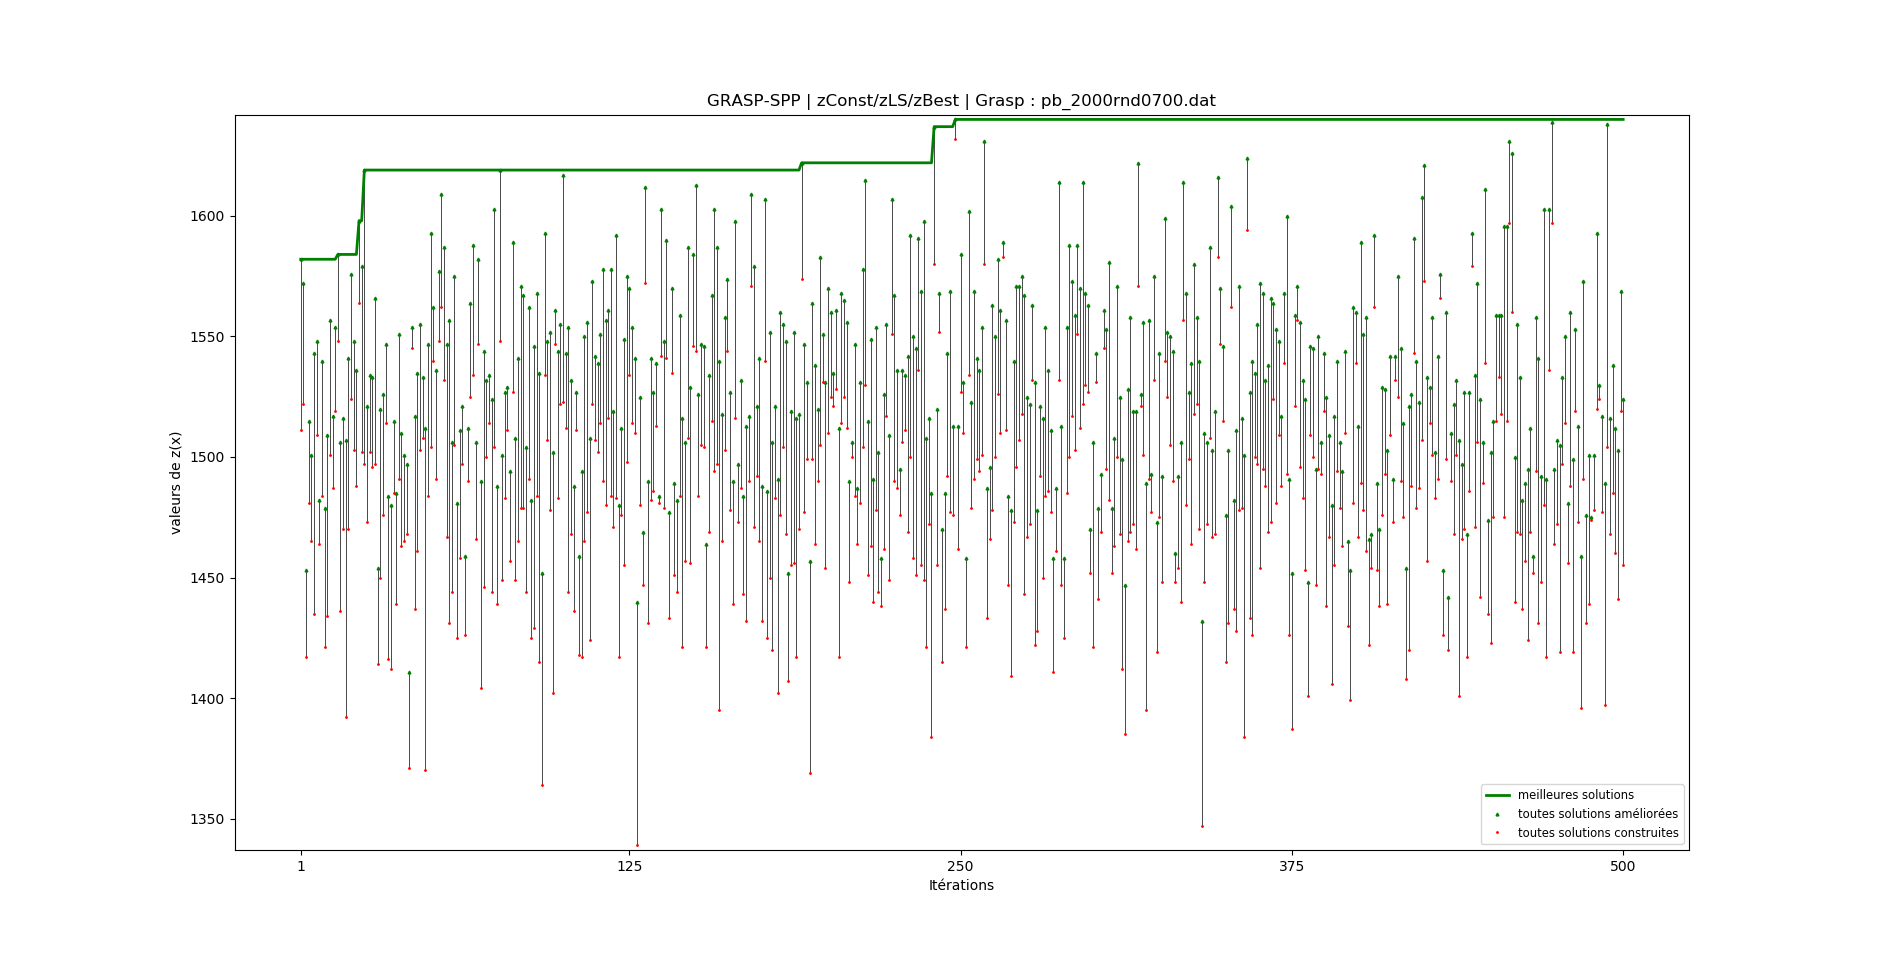
\includegraphics[scale=0.37]{fig/Grasppb2000rnd0700.png}
    %\caption{patate}
    \label{fig:grasp2000rnd0700}
  \end{figure}
\end{example}



Pourcentage de précision de Grasp sur 10 instances pour différents $\alpha$ pendant 10 secondes
\begin{center}
    \begin{tabular}{|c|c|c|c|c|c|c|c|c|c|c|}  
    \hline
    nom de l'instance &  $\alpha=0.2$ &  $\alpha=0.4$ &  $\alpha=0.5$ &  $\alpha=0.6$ & $\alpha=0.7$ &  $\alpha=0.8$ &  $\alpha=0.9$ &  $\alpha=0.95$ \\
     \hline
     pb1000rnd0300 & 76.25 & 82.9 & 83.36 & 86.23 & 86.69 & \textcolor{red}{89.41} & 87.29 & 88.2\\
     \hline
     pb1000rnd0700 & 93.81 & 94.07 & \textcolor{red}{96.24} & 95.18 & 95.13 & 95.04 & 93.63 & 93.01\\
     \hline
     pb100rnd0500 & \textcolor{red}{100} & 100 & 100 & 100 & 99.06 & 98.12 & 98.12 & 98.12\\
     \hline
     pb2000rnd0700 & 78.63 & 88.63 & 88.4 & 88.63 & \textcolor{red}{90.78} & 90.56 & 89.56 & 88.07\\
     \hline
     pb200rnd0100 & \textcolor{red}{99.28} & 98.8 & 97.84 & 100 & 96.88 & 96.88 & 95.91 & 95.19\\
     \hline
     pb200rnd0300 & 96.03 & 96.58 & \textcolor{red}{96.99} & 96.17 & 96.85 & 96.58 & 96.31 & 95.76\\
     \hline
     pb200rnd0700 & 98.9 & \textcolor{red}{99.7} & 99.5 & 98.71 & 98.8 & 98.21 & 97.71 & 96.41\\
     \hline
     pb200rnd0900 & 99.62 & \textcolor{red}{100} & 99.85 & 99.85 & 99.85 & 99.62 & 99.62 & 99.55\\
     \hline 
     pb500rnd0700 & 97.63 & 97.72 & 98.6 & 99.21 & \textcolor{red}{99.74} & 98.69 & 96.67 & 96.67\\
     \hline 
     pb500rnd0900 & 97.54 & 98.75 & 98.88 & 98.66 & 98.93 & \textcolor{red}{98.97} & 98.88 & 98.52\\
     \hline
    \end{tabular}
\end{center}


\paragraph{Remarques : }
\begin{itemize}
\item On observe que le choix du paramètre est important et peut entrainer un écart de précision de plus de 10\%.

\item On remarque aussi que les grandes instances et les instances particulières qui étaient lentes sur les k-p échanges font moins d'itérations de Grasp que les rapides, et donc qu'il est important de régler le $N_{\alpha}$ en conséquence. 
\end{itemize}


\vspace{5mm}
\noindent
\fbox{
  \begin{minipage}{0.97 \textwidth}
    \begin{center}
      \vspace{1mm}
        \Large{Expérimentation numérique de ReactiveGRASP}
      \vspace{1mm}
    \end{center}
  \end{minipage}
}
\vspace{2mm}

%\noindent Présenter le protocole d'expérimentation (env. matériel; budget de calcul; condition(s) d'arrêt).

%\noindent Rapporter graphiquement vos résultats selon $\hat{z}_{min}$, $\hat{z}_{max}$, $\hat{z}_{moy}$ mesurés à intervalles réguliers (exemple de pas de 10 secondes).

%\noindent Rapporter l'apprentissage du paramètre $\alpha$ réalisé par ReactiveGRASP, les valeurs saillantes établies.

%\noindent Présenter sous forme de tableau les résultats finaux obtenus pour les 10 instances sélectionnées.

\begin{example}
  Une éxecution du réactive Grasp sur le Pb 2000rnd0700
  \begin{figure}[htb!]
    \centering
    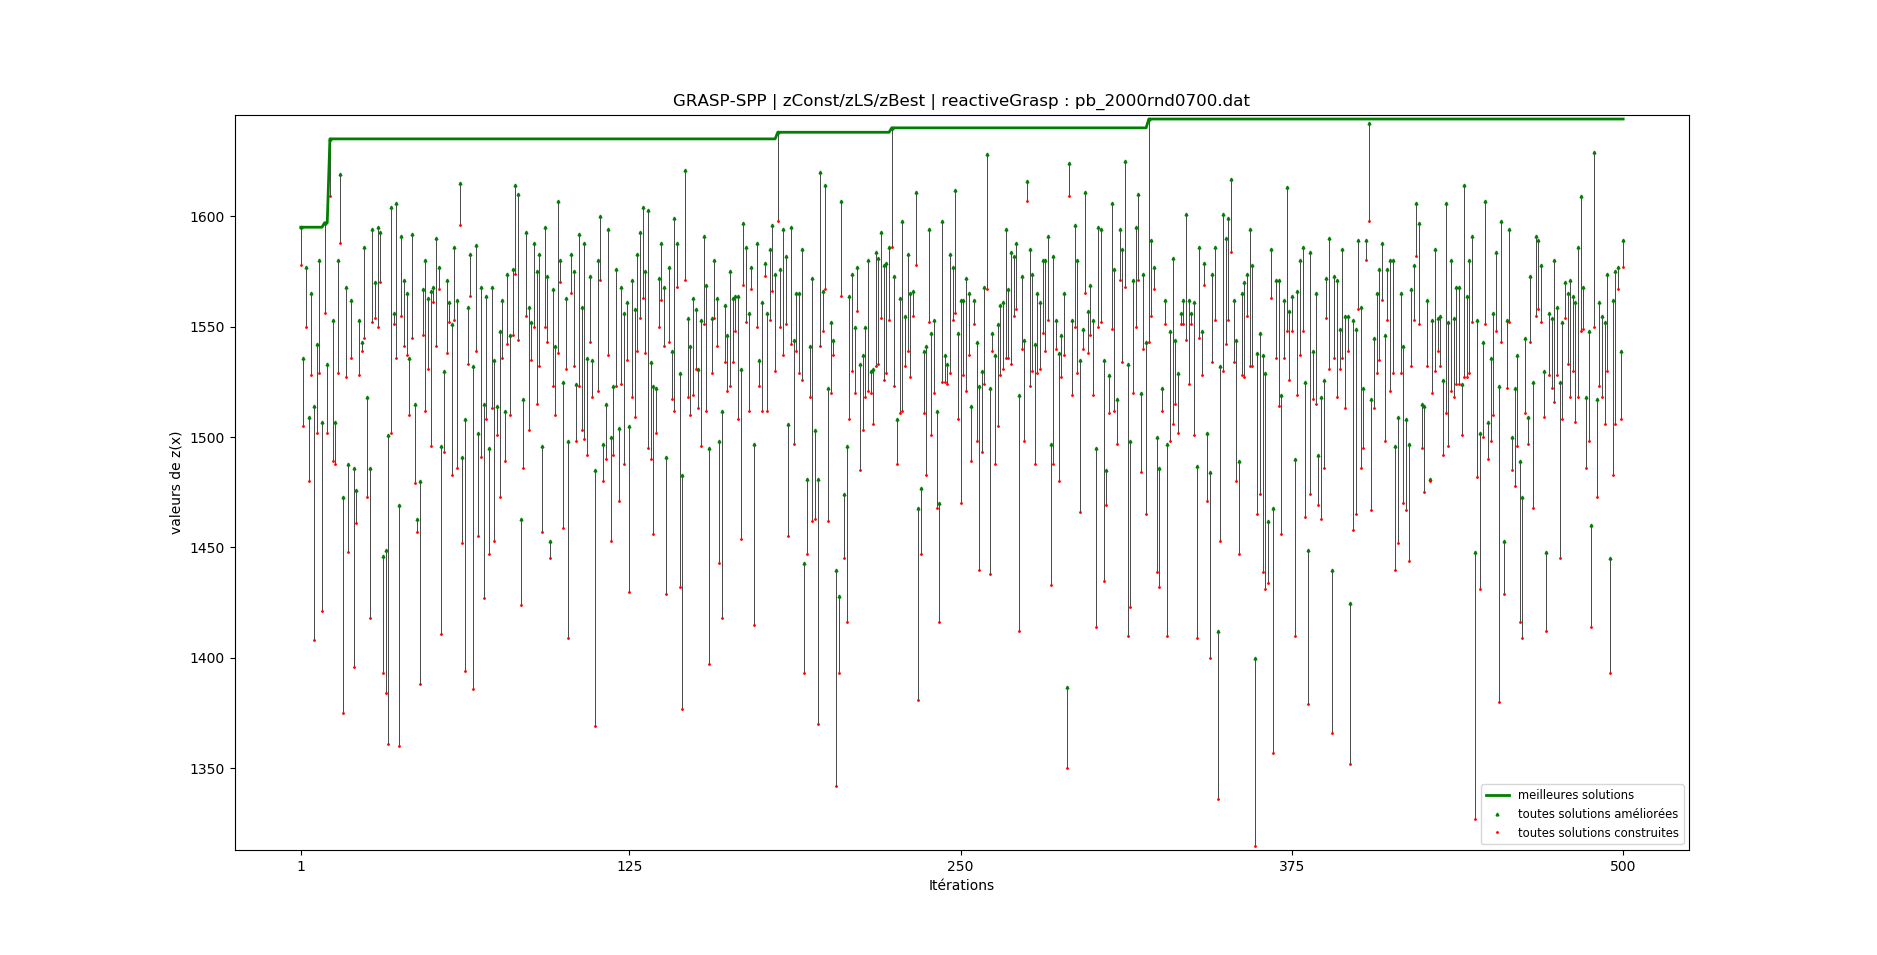
\includegraphics[scale=0.37]{fig/Na=100,nb=500/pb2000rnd0700.png}
    %\caption{patate}
    \label{fig:reactive2000rnd0700}
  \end{figure}

  \vfill
  \break
  
  Distribution finale d'$\alpha$ :
  \begin{figure}[htb!]
    \centering
    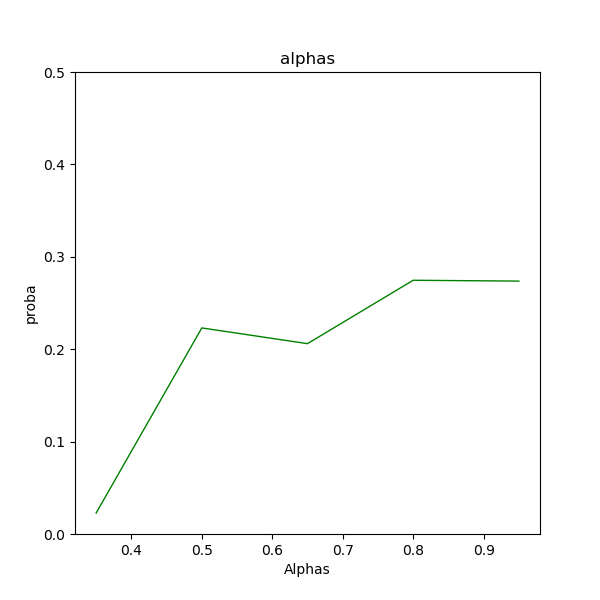
\includegraphics[scale=0.5]{fig/Alpha1.png}
    %\caption{patate}
    \label{fig:alpha1}
  \end{figure}
\end{example}


Pourcentage de précision de Réactive Grasp sur 10 instances pour $\alpha$ dans $[0.35,0.5,0.65,0.8,0.95]$. Avec $N_{\alpha} = 100$ sur 500 itérations.
\begin{center}
    \begin{tabular}{|c|c|c|}  
    \hline
    nom de l'instance & $\alpha$ dominant & précision \\
     \hline
     pb1000rnd0300 & 0.8 & 90.92\% \\
     \hline
     pb1000rnd0700 & 0.65 & 96.19\%\\
     \hline
     pb100rnd0500 & 0.5 & 100\%\\
     \hline
     pb2000rnd0700 & 0.8 & 90.78\%\\
     \hline
     pb200rnd0100 & 0.95 & 98.8\%\\
     \hline
     pb200rnd0300 & 0.95 & 96.31\%\\
     \hline
     pb200rnd0700 & 0.65 & 98.41\%\\
     \hline
     pb200rnd0900 & 0.95 & 100\%\\
     \hline 
     pb500rnd0700 & 0.95 & 98.95\%\\
     \hline 
     pb500rnd0900 & 0.95 & 99.02\%\\
     \hline
    \end{tabular}
\end{center}

% 
alphas : [0.55,0.65,0.75,0.85,0.95]

data/pb_1000rnd0300.dat

alpha dominant : 0.85
accuracy: 93.65%

  data/pb_1000rnd0700.dat

alpha dominant : 0.75
accuracy: 95.71%

  data/pb_100rnd0500.dat

alpha dominant : 0.55
accuracy: 99.84%

  data/pb_2000rnd0700.dat

alpha dominant : 0.85
accuracy: 93.15%

  data/pb_200rnd0100.dat

alpha dominant : 0.95
accuracy: 96.88%

  data/pb_200rnd0300.dat

alpha dominant : 0.95
accuracy: 96.85%

  data/pb_200rnd0700.dat

alpha dominant : 0.65
accuracy: 98.71%

  data/pb_200rnd0900.dat

alpha dominant : 0.95
accuracy: 99.7%

  data/pb_500rnd0700.dat

alpha dominant : 0.85
accuracy: 99.12%

  data/pb_500rnd0900.dat

alpha dominant : 0.85
accuracy: 98.88%



\paragraph{Remarques : }
\begin{itemize}
\item On retrouve sensiblement les mêmes précisions qu'avec les meilleurs Grasp et les $\alpha$ dominants correspondent, sauf sur les instances où le paramètre n'avait pas beaucoup d'influence (par exemple le pb 200rnd0300)
\item On a donc réussi à régler le paramètre $\alpha$ mais au prix d'une discrétisation arbitraire et d'un nouveau paramètre $N_{\alpha}$.
\end{itemize}


\vspace{5mm}
\noindent
\fbox{
  \begin{minipage}{0.97 \textwidth}
    \begin{center}
      \vspace{1mm}
        \Large{Eléments de contribution au bonus}
      \vspace{1mm}
    \end{center}
  \end{minipage}
}
\vspace{2mm}

\paragraph {Path-relinking} \noindent

Le principe du path-relinking\cite{path} est de pousser plus loin les recherches de solutions de bonne qualité à travers l'espace des solutions. Nous partons de solutions trouvées par plusieurs lancés du reactiveGrasp sur une même instance. Nous essayons de partir d'une solution pour rejoindre l'autre en réalisant un swap aléatoire sur les variables qui ont des valeurs différentes dans les deux solutions, tout en restant dans l'espace de solutions admissibles. Sur ce parcours entre les deux, dès qu'une solution trouvée par un swap semble prometteuse (défini arbitrairement), nous réalisons une descente profonde pour rechercher s'il n'y a pas un optimimum, au moins local, plus intéressant.

Observations :  On remarque d'une part, peu d'améliorations sur les petites instance et un path relinking qui boucle sur certaines combinaisons de solutions de départ. Mais d'autre part des améliorations conséquentes (jusqu'à 5\%) sur certaines grosses instances.

Nous avons essayé deux définitions de solution prometteuse, soit on considérait toutes les instances admissibles trouvées prometteuses sans distinction soit on ne prenait que les solutions dont la fonction objectif était supérieur à la solution de départ.

\paragraph {Parallélisme} \noindent


Le parallélisme consiste à envoyer plusieurs parties de nos calculs aux différents coeurs d'une machine et de mutualiser les résultats pour gagner du temps.
Cette méthode se révèle très pratique pour une application du path relinking. On calcule en parallèle deux solutions avec reactive Grasp et on les utilise ensuite pour faire un path relinking.
En julia on utilise la fonction @parallel pour paralléliser les appels de reactive Grasp et la fonciton append! comme réducteur pour concaténer nos solutions dans un vecteur de solutions.

Nous n'avons utilisé le parralélisme seulement pour le path-relinking mais il serait possible de le mettre en oeuvre avec le GRASP et le ReactiveGRASP pour réduire les temps de calculs.

%\noindent \prof{Présenter vos contributions aux aspects proposés en bonus.}



\vspace{5mm}
\noindent
\fbox{
  \begin{minipage}{0.97 \textwidth}
    \begin{center}
      \vspace{1mm}
        \Large{Discussion}
      \vspace{1mm}
    \end{center}
  \end{minipage}
}
\vspace{2mm}


Le problème du Grasp est que son paramètre est arbitraire et peut beaucoup jouer sur la qualité de la solution.
Le Réactive grasp résoud ce problème en apprenant sur les données le $\alpha$ le mieux adapté à celles-ci. Néanmoins, cet apprentissage a besoin d'être réglé aussi et une fois fait, certaines instances restent peu propices à cet apprentissage.
Le path-relinking et le parallélisme permettent d'améliorer les solutions en peu de temps de calculs sur les grandes instances. 


%\noindent \prof{Tirer des conclusions en comparant les résultats collectés avec vos deux variantes de métaheuristiques.}


%\noindent \prof{Quelles sont les recommandations que vous émettez à l'issue de l'étude et avec quelle variante continuez vous l'aventure des métaheuristiques?}


\paragraph{Remarques : }
\begin{itemize}
\item On observe que nos heuristiques sont globalement très mauvaises en temps (par rapport au simplexe) sur les données qui ont des fonctions objectifs uniformes (où toutes les variables ont le même poids)
\item On remarque aussi que la meilleure solution est parfois trouvée par les deux résolutions parallèles. Cela rend le path relinking inutile. On peut en conclure que limiter les grasp par leur nombre d'itérations est plus sécurisant quant à l'efficacité de l'heuristique. Malheureusement, la limite réelle est souvent temporelle.
\end{itemize}

Pour les heuristiques à paramètres, il faut être conscient qu'un bon réglage des paramètres est essentiel pour un bon fonctionnement des heuristiques. Ce réglage peut être fait par l'observation et les tests ou par un apprentissage automatisé. 


\vfill
\break


\bibliographystyle{plain}

\bibliography{xavier}
  % decommenter lors de la remise du DM2 uniquement

% -----------------------------------------------------------------------------------------------------------------------------------------------------

% =====================================================================================
% Document : rendu du DM2
% Auteur : Xavier Gandibleux
% Année académique : 2018-2019

\section*{Livrable du devoir maison 3 : \\ Battle of metaheuristics}

%
% -----------------------------------------------------------------------------------------------------------------------------------------------------
%

\vspace{5mm}
\noindent
\fbox{
  \begin{minipage}{0.97 \textwidth}
    \begin{center}
      \vspace{1mm}
        \Large{Présentation succincte des choix de mise en \oe uvre de la métaheuristique concurrente à GRASP appliquée au SPP}
      \vspace{1mm}
    \end{center}
  \end{minipage}
}
\vspace{2mm}


%\prof{Présenter l'algorithme mis en oeuvre. Illustrer sur un exemple didactique (poursuivre avec l'exemple pris en DM1). Présenter vos choix de mise en oeuvre.}

Nous avons choisi d'implémenter les méthodes de recherche Tabou (TS) et de Recuit Simulé (SA). 
Nous présentons donc chacune des deux méthodes dans les paragraphes suivants :

\paragraph{Recherche Tabou}

Rappel de la méthode :

La méthode Tabou, ou Tabu Search, est une méthode déterministe de recherche d'optimum. L'idée est de chercher la meilleure solution possible d'un problème(ici un SPP) en parcourant l'ensemble des solutions, sans rester bloqué dans un optimum local comme pour une plus profonde descente. Cela signifie donc avancer dans l'espace des solutions sans pouvoir immédiatement revenir en arrière. \\
Pour démarrer, l'algorithme part d'une solution admissible et cherche son meilleur voisin. (Cette démarche s'applique même si le voisin trouvé est moins bon que la solution actuelle). Une fois le meilleur voisin trouvé, le mouvement réalisé est enregistré comme mouvement tabou, c'est-à-dire inutilisable pour une certaine période de temps (un nombre de tours de boucles dans les faits). Ce meilleur voisin est ensuite comparé avec la meilleure solution trouvée jusqu'à maintenant, et la meilleure des deux est gardée en mémoire. On se place ensuite sur le meilleur voisin trouvé pour inspecter son voisinage. La même démarche que précédemment sera prise, avec ceci près que le meilleur voisin trouvé ne devra pas être atteint avec un mouvement actuellement tabou. Au fur et à mesure que l'algorithme se déroule, le nombre de mouvement inutilisable augmente. Pourtant, cela pourrait empêcher de revenir sur des solutions qui ont été vu mais qui permettent de passer sur une partie de l'espace des solutions non visitée. Pour cette raison, il existe un temps ou nombre de boucles au bout desquels un mouvement redevient utilisable.\\
Dans cette méthode, la liste/tableau de mouvement Tabou est l'élément essentiel pour permettre de se déplacer dans une grande partie de l'espace des solution et d'éviter de retomber dans un optimum local déjà visité au prochain tour de boucle. La meilleure solution sera donc celle retenue lors du parcours de l'espace des solutions, à l'issue d'un nombre d'itérations ou temps limite.

Une amélioration de l'algorithme Tabu Search, nommé Reactive TS, est de faire varier la longueur de la liste tabou, ou autrement dit la durée d'interdiction d'un mouvement en fonction d'un apprentissage sur les données.
En effet, il est possible de voir l'algorithme boucler et rester dans une même partie de l'espace parce qu'il ne peut en sortir pour cause de mouvements tabous. L'idée est donc de détecter ces cas et d'autoriser à nouveau ces mouvements, pour sortir de ce cyclage.



Implémentation :

Toujours en utilisant la structure de données avec les vecteurs de vecteurs, nous avons aussi repris deux fonctions du DM1:
\begin{itemize}
    \item le glouton déterministe le plus efficace (gloutonVxV)
    \item la plus profonde descente, où l'on incorpore la notion de mouvement tabou (pour la version 2 du tabou)
    \item la fonction d'admissibilité
\end{itemize}

Dans l'implémentation du calcul des voisins, nous avons choisis, pour des raison d'efficacité, de parcourir les voisins en retenant le plus petit au fur et à mesure au lieu de calculer l'ensemble des voisins puis de choisir le plus petit.


Remarques :

Dans un premier temps, nous avions choisi, pour optimiser le temps d'exécution, de représenter la liste tabou dans une matrice (dans l'idéal, cette matrice serait triangulaire). Nous n'utilisions alors qu'un mouvement d'1-1 échange. Cependant, pour les instances qui ont des fonctions objectifs avec des coûts tous similaires, cela ne permet aucune amélioration. Nous avons donc réalisé une seconde implémentation.

Seconde implémentation (tabou3) :

Pour améliorer notre tabou, nous avons décidé d'augmenter son voisinage en ajoutant les 2-1 et 0-1 échanges. Nous avons donc repris les échanges utilisés par le grasp en y ajoutant la notion de mouvements tabou.

Ce nouveau voisinage permet de mieux explorer l'espace des solution mais en contrepartie, nous avons une représentation des mouvements tabou moins précise. En effet, dans notre liste (représentée dans un tableau pour une question d'efficacité), nous ne retenons que les variables qui ont récemment été mise à 1. Cela ne correspond pas à un mouvement mais à cause de l'ajout des nouveaux voisinages, la représentation de la liste tabou pouvait devenir très lourde. Nous avons donc choisi de la rendre moins précise.

Ce choix a pour effet qu'un tabou représente plusieurs mouvements possibles et donc peut potentiellement empêcher un mouvement inédit améliorant.


\paragraph{Recuit simulé}

Rappel de la méthode :

Le Recuit Simulé est une méthode stochastique qui recherche le meilleur voisin possible mais en contrôlant au fur et à mesure la direction de recherche dans l'espace des solutions.

Le Recuit Simulé consiste à se déplacer aléatoirement dans un voisinage en acceptant parfois certaines solutions détériorantes afin de ne pas rester coincé dans un voisinage. Ce contrôle se fait en utilisant un schéma de refroidissement : une fonction simulant le refroidissement d'un alliage est utilisée. Cette fonction décroit exponentiellement.
Le principe est le suivant : à partir d'une solution, on choisit au hasard l'un de ces voisins admissibles. Un nombre p est tirée au hasard entre 0 et 1. La solution voisine S' est retenue si la solution est améliorante ou bien si le nombre p est inférieur à la fonction de refroidissement (qui varie en fonction de la température et de la différence entre la meilleure solution et l'actuelle). Si la solution est acceptée, on la compare ensuite avec la meilleure solution en mémoire. Sinon, on garde la solution S. Enfin, la température T est mise à jour. Cette démarche se répète ensuite sur la solution retenue jusqu'à une limite de temps ou bien un certain nombre de voisins refusés.

Implémentation :

Nous avons remarqué qu'utiliser un seul swap comme voisinage était une mauvaise idée, car toutes les instances à fonction objectif composées uniquement de coûts réduits à 1 ne peuvent pas être améliorées. Nous avons donc élargi le voisinage de la manière suivante :
Le voisinage choisi oscille aléatoirement entre un 1-1échange, un 0-1 et un 1-0 à respectivement 80\%, 10\%,et 10\% de chance.
De cette manière, l'algorithme ne reste pas bloqué sur les instances à fonction objectifs spéciales ou tout autre voisinage avec une configuration complexe.


Dans cette méthode, il y a donc 3 (voire 4) paramètres à régler :
\begin{itemize}
    \item la température $ T_0 $ : En partant au début d'une température très grande, on décide d'accepter beaucoup de solution dégradante pour ensuite être de plus en plus restrictifs au fur et à mesure que cette température baissera.
    \item le palier L : On note que la mise à jour de la température se fait en fonction de la température initiale $ T_0 $ mais aussi de la taille du palier donnée en entrée. Un palier très long est plus longtemps permissif envers les solutions de mauvaises qualités.
    \item Le coefficient de refroidissement $ \alpha $ : Ce coefficient est celui qui permet de régler la vitesse de convergence de la fonction de refroidissement vers 0. 
    \item Le nombre de refus maximal autorisé (éventuel critère limite): Dans notre cas, pour pouvoir comparer avec le TS avec une même contrainte de temps, nous avons peu joué dessus.
\end{itemize}


%
% -----------------------------------------------------------------------------------------------------------------------------------------------------
%

\vspace{5mm}
\noindent
\fbox{
  \begin{minipage}{0.97 \textwidth}
    \begin{center}
      \vspace{1mm}
      \Large{Expérimentation numérique comparative \\
        Reactive GRASP + Path Relinking VS Recherche Tabou VS Recuit Simulé}
      \vspace{1mm}
    \end{center}
  \end{minipage}
}
\vspace{2mm}

%\prof{\noindent Présenter le protocole d'expérimentation (environnement matériel; budget de calcul; condition(s) d'arrêt; réglage des paramètres).}

Les conditions pour les expérimentations sont les suiavntes : 
Les codes sont réalisés sous Julia 0.6.4 en mode mutlicoeur avec la commande : julia -p $<$nombres de coeurs$>$

L'ensemble des programmes ont été réalisé en julia 0.6.4 et les tests ont été effectués avec un pc acer sous ubuntu18 avec les caractéristiques suivantes : 
\begin{itemize}
\item RAM : 4 Gio
\item CPU : Intel® Core™ i3-7130U CPU @ 2.70GHz × 4 
\item GPU : Intel® HD Graphics 620 (Kaby Lake GT2)
\end{itemize}


\paragraph{Protocole}
Des tests sont réalisées avec les deux méthodes Tabu Search, Simulated Annealing et sont comparées aux résultats du ReactiveGrasp.
Pour chaque instance, on lance des tests avec chaque méthode, et en essayant avec deux temps limites possibles 3 et 10 secondes.


%\prof{Rapporter graphiquement vos résultats selon $\hat{z}_{min}$, $\hat{z}_{max}$, $\hat{z}_{moy}$ mesurés à intervalles réguliers (exemple de pas de 10 secondes).}
\begin{example}
  Une éxecution du Recuit Simmulé
  \begin{figure}[htb!]
    \centering
    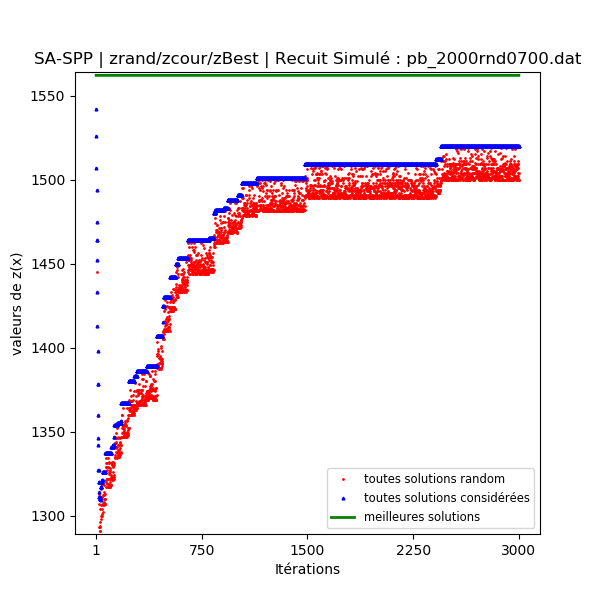
\includegraphics[scale=0.5]{fig/recuit.png}
    %\caption{patate}
    \label{fig:recuit}
  \end{figure}
\end{example}

\begin{example}
  Une éxecution de la Recherche Tabou
  \begin{figure}[htb!]
    \centering
    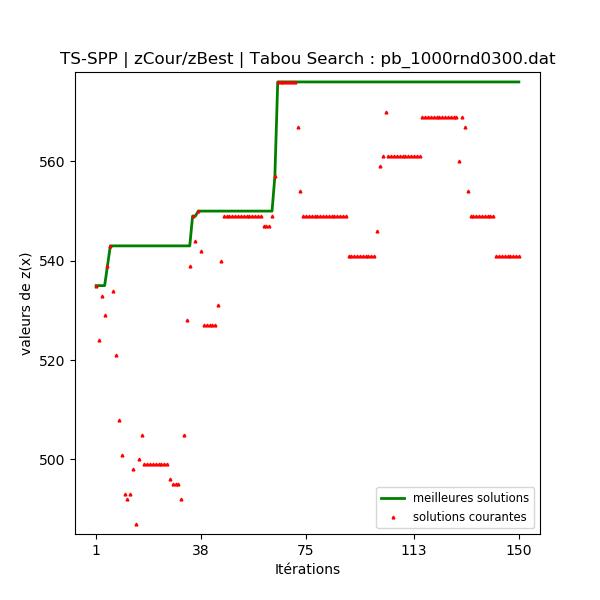
\includegraphics[scale=0.5]{fig/tabou.png}
    %\caption{patate}
    \label{fig:recuit}
  \end{figure}
\end{example}

On observe que globalement, nos solutions obtenues par les gloutons et servant de solution de départ pour les autres méthodes sont de bonne qualité. C'est pour cette raison que le recuit simulé a du mal à l'améliorer dans l'exemple ci-dessus. En fait, cela est aussi vrai pour plusieurs instances, les TS et SA n'arrive pas toujours à améliorer car la solution de départ est très bonne.


%\prof{Rapporter l'étude de l'influence du paramètre $\alpha$.}
Paramétrage du Tabu Search : Lorsque la tabou liste est longue, si on tombe dans une phase de cyclage (c'est-à-dire un cas où il est difficile de sortir d'une partie du voisinage), elle donne l'occasion d'en sortir. A l'inverse, si elle est courte, il y a le risque de cycler et de rester dans la même zone indéfiniment. On remarque qu'une tabou liste de taille 25 est un bon compromis pour éviter le cyclage et en même temps parcourir l'ensemble de l'espace. Bien sûr, ce réglage correspond au voisinage que nous avons choisi.

Paramétrage du Simulated Annealing : Nous avons étudié les trois paramètres sur toutes les instances. Nous en donnons un exemple ici, sur l'instance : 1000rnd0700
Le paramétrage de référence : L = 6, $T_0$ = 150, $\alpha$ = 0.4
On part d'un glouton à 92.83\% de la solution.
\begin{center}
    \begin{tabular}{|c|c|c|c|}  
    \hline
    paramètre changé & sa valeur & Qualité de solution &  Observations générales \\
     \hline
     ... & ...  & 94.64\% & référence\\
     \hline
     L & 3 & 93.05\% & descente trop rapide pour tomber sur une bonne solution\\
     \hline
     L & 10 & 92.83\% & affinage ralenti, très peu de restriction\\
     \hline
     $T_0$ & 50 & 93.1\% & pas assez de liberté\\
     \hline
     $T_0$ & 500 & 94.25\% & trop de temps à refroidir\\
     \hline
     $\alpha$ & 0.9 & 92.83\% & pas assez agressif \\
     \hline
     $\alpha$ & 0.15 & 94.56\% & convergence trop rapide \\     
     \hline
   \end{tabular}
\end{center}

Concernant le paramètre $T_0$ , ces observations dépendent aussi du temps/nombre d'itérations limite accordées. En effet, une chaleur très élevée peut donner de bons résultats si on lui donne beaucoup de temps pour refroidir et arriver dans la phase de restrictions des solutions.
On note cependant que le paramétrage pourrait être meilleur, en prenant en compte, par exemple, du nombre de variables et de contraintes de l'instance sur laquelle la méthode est appliquée.

%\prof{Présenter sous forme de tableau les résultats finaux obtenus pour les 10 instances sélectionnées.}

\begin{center}
    \begin{tabular}{|c|c|c|c|c|}  
    \hline
    nom de l'instance &  Tabou Search & Simmulated Annealing & Reactive Grasp\\
     \hline
     pb1000rnd0300 & 87.14\% & 79.43\% & 85.17\% \\
     \hline
     pb1000rnd0700 & 95.22\% & 93.67\% & 94.65\% \\
     \hline
     pb100rnd0500 & 97.97\% & 97.97\% & 100\% \\
     \hline
     pb2000rnd0700 & 90.83\% & 87.58\% & 91\% \\
     \hline
     pb200rnd0100 & 94.95\% & 88.22\% & 96.88\% \\
     \hline
     pb200rnd0300 & 95.9\% & 94.25\% & 96.72\% \\
     \hline
     pb200rnd0700 & 96.81\% & 95.12\% & 99.4\% \\
     \hline
     pb200rnd0900 & 99.55\% & 99.55\% & 99.92\% \\
     \hline 
     pb500rnd0700 & 97.63\% & 97.11\% & 98.69\% \\
     \hline 
     pb500rnd0900 & 98.39\% & 99.15\% & 98.79\% \\
     \hline
    \end{tabular}
\end{center}

Paramètres sur 3 sec :
\begin{itemize}
\item R-Grasp : $N_{\alpha} = 10$ et $V_{\alpha} = [0.35,0.5,0.65,0.8,0.95]$
\item TS : Tabou lenght = 25
\item SA : L = 6, $T_0$ = 150, $\alpha$ = 0.4
\end{itemize}

On peut comparer les heuristiques en comptant le nombre de fois où elles ont obtenues un meilleur résultat, pour un même temps donné. Cependant, il ne faut pas oublier que les solutions trouvées par ces trois méthodes restent assez proches. Nous remarquons que les méthodes aléatoires peuvent occasionnellement dépasser les solutions du Tabou Search. Ainsi, nous pouvons noter que le Tabu Search, en une fois nous permet de trouver une très bonne solution. Cependant, avec plusieurs tentatives et un bon tuning de paramètres, comme pour le Grasp, il devient possible de trouver des solutions encore meilleures mais de manière beaucoup plus coûteuse. 
\begin{center}
  Médailles pour les dix instances : \\
    \begin{tabular}{|c|c|c|c|}  
    \hline
    heuristique & ---Or--- & ---Argent--- & ---Bronze---\\
    \hline
    TABOU & 3 & 7 & 3 \\
    \hline
    SA    & 1 & 3 & 9\\
    \hline
    GRASP & 7 & 3 & 1\\
    \hline
    \end{tabular}
\end{center}

Des tests sont lancés pendant 3 et 10 secondes avec une TL de 10 sans remarquer de différences dans les solutions. La version ci-dessous correspond à des tests avec un temps limite de 3 secondes. Nous remarquons que Grasp est le meilleur sur ce groupe d'instances. Cela s'explique par l'apprentissage  du paramètre $\alpha$ et l'ajout du path-relinking. Les deux autres méthodes méritent encore quelques modifications pour les parfaire. Pour le Tabu Search, il serait bon de réaliser une implémentation non pas avec une matrice des variables changées mais bien une liste de mouvements. Pour le Simulated Annealing, il serait possible d'améliorer les résultats avec un tuning des paramètres en prenant en compte le nombre de variables et de contraintes. Il est aussi important de noter que les méthodes aléatoires dépendent des graines choisies et, on peut se demander si, selon celles choisies, il peut-être possible de tomber plus facilement sur une solution meilleure que celle du Tabu Search par hasard. En effet, plusieurs tentatives avec les mêmes paramètres avec le SA ont montré qu'il était possible de dépasser occasionnellement le Tabu Search. \\
Dans un test sur l'ensemble des instances, on remarque que le TS a autant de succès que le ReactiveGrasp, et le SA donne aussi de bons résultats. Respectivement, ces méthodes détiennent les meilleures solutions pour 38, 39 et 21 instances. Nous pouvons nous demander si chaque méthode est bonne pour un type de sous-problème donné. 

%
% -----------------------------------------------------------------------------------------------------------------------------------------------------
%

\vspace{5mm}
\noindent
\fbox{
  \begin{minipage}{0.97 \textwidth}
    \begin{center}
      \vspace{1mm}
        \Large{Discussion}
      \vspace{1mm}
    \end{center}
  \end{minipage}
}
\vspace{2mm}


%\prof{Tirer des conclusions en comparant les résultats collectés avec vos deux métaheuristiques.}
Conclusion globale :

En remarque globale, on observe que le choix du voisinage est primordial pour l'efficacité d'une heuristique sur un problème. Nous remarquons aussi qu'une heuristique prise pour un type de (sous-)problème est plus optimisé et donne de meilleurs résultats. En effet, nos premières tentatives de TS et SA étaient bonnes pour des instances avec des fonctions objectifs avec des coûts réduits non tous égaux à 1. Nous pouvons remarquer que l'heuristique TS a l'avantage de donner dès le premier lancement une solution de bonne qualité en général, alors que celles stochastiques nécessitent un paramétrage.

Pistes d'améliorations :

Comme noté précédemment, nous supposons que les deux heuristiques TS et SA peuvent encore être améliorées, via ,respectivement, une liste des mouvement et un apprentissage des paramètres par rapport aux nombres de variables et de contraintes notamment. 

Comme amélioration, nous avons essayé de faire un path-relinking sur les solutions du TS et du SA puis un deuxième entre cette nouvelle solution et celle du reactive grasp. De cette manière, nous espérions construire une très bonne solution mais malgré plusieurs tests avec plusieurs temps d'arrêts différents, nous n'avons pas observé d'amélioration.

Il pourrait aussi être intéressant d'essayer de trouver un moyen pour avoir une borne nous indiquant l'optimalité à une erreur près. 


%\prof{Quelles sont les recommandations que vous émettez à l'issue de l'étude ?}

L'optimisation des heuristiques se fait à tous les niveaux : sur les structures de données, sur les caractéristiques du langage, et sur une l'implémentation intelligente de l'algorithme en évitant toutes opérations coûteuses. On remarque vite l'avantage d'une heuristique déterministe pour l'analyse des résultats. Afin d'obtenir une solution de bonne qualité, il est important de bien choisir une heuristique adaptée au problème, et de bien analyser les différents types d'instances à résoudre.





 % decommenter lors de la remise du DM3 uniquement



\end{document}

